\section{Parameter estimation and Bayesian lens reconstruction}
\label{sec:pe}
The benchmark of Section~\ref{sec:results} uses a simplified, SNR-based model of the GW measurements (Section~\ref{sec:gwmeas}) and estimators trained on simulations. Here we test both ingredients on a random subset of systems, with equal numbers per lens family and scenario: the SNR-based model against joint Bayesian parameter estimation (PE) of both images from simulated detector data (strain), and the trained estimators against conventional Bayesian lens reconstructions that use the same observables and priors, with and without the strain data.

\subsection{Joint parameter estimation of lensed image pairs}
\label{sec:jointpe}
We drew 15 selected systems per lens family and scenario (120 in total) at random from catalogues generated with the same configuration as the benchmark, excluding the lightest detector-frame binaries whose analysis segment would exceed 256\,s. For each system both images were injected into independent stationary Gaussian noise with the A+/AdV (O5-like) or ET-D power spectral densities, using the \textsc{IMRPhenomXHM} waveform with higher harmonics \citep{garciaquiros2020xhm}, the Morse phase of each image and the antenna patterns at each arrival time. We sampled the joint posterior of the shared source parameters (chirp mass, mass ratio, aligned spins, sky position, polarisation, inclination, phase, apparent distance and arrival time of image $A$) and the lensing parameters $\ln(\mu_B/\mu_A)$, the delay and the two Morse indices, with \textsc{bilby} \citep{ashton2019bilby}, the \textsc{dynesty} nested sampler \citep{speagle2020dynesty} and relative binning \citep{zackay2018relbin,krishna2023relbin}, which speeds up the likelihood by expanding each waveform around a reference waveform, here the injected signal. Where the relative-binning log-likelihood exceeds that of the reference waveform by more than 50, which signals a failure of the approximation because the reference lies close to the maximum-likelihood point, we evaluate the exact likelihood instead. We analysed every system twice: with a free sky position, as in a GW-only analysis, and with the sky position fixed to that of the host, which is known to sub-arcsecond precision once the lens system is identified in imaging, as the benchmark assumes. The apparent-distance prior is uniform in volume. We used 150 live points and the acceptance-walk method of \textsc{bilby}, with 30 accepted Markov-chain steps for each new live point. For the free-sky ET posteriors, which have several separated solutions, this is not sufficient (see below), which is one reason we base the comparison with the SNR-based model on the known-sky analyses. Each system has its own noise realisation, fixed by a seed derived from its identifier, so that the GW-only and GW+EM analyses below see identical data. A run takes of order 10--30 CPU hours.

Fig.~\ref{fig:pe} compares the joint-PE posteriors with the SNR-based model of Section~\ref{sec:gwmeas}. With the host sky position, the 90 per cent intervals of $\ln(\mu_B/\mu_A)$ and of the apparent distance of image $A$ contain the truth for 52 and 50 of the 60 ET systems (coverage $0.87\pm0.04$ and $0.83\pm0.05$, binomial errors), and the free-sky O5 intervals for 55 and 53 of 60 ($0.92\pm0.04$ and $0.88\pm0.04$). The probability integral transforms are consistent with uniform (Kolmogorov--Smirnov $p=0.06$ for ET and $0.09$ for O5), and the difference of Morse indices is identified with posterior probability above 0.5 in all ET and in 59 of 60 O5 systems. The PE uncertainties are smaller than those of the SNR-based model: by a factor 0.91 for $\ln(\mu_B/\mu_A)$ in O5 and 0.41 in ET, and by factors 0.67 and 0.44 for $\ln D_{{\rm app},A}$. For ET the SNR-based model is therefore conservative. The joint PE fixes the source parameters that the two images share, and the higher harmonics break part of the inclination--distance degeneracy that dominates the catalogue-calibrated apparent-distance errors, so the median $\sigma_{\ln D}$ is 0.10 for ET rather than 0.24.

Free-sky ET analyses fail in a characteristic way. A single ET site constrains the sky position poorly, and the sky position, the polarisation and the Morse phase of each image are partly degenerate. With 150 live points the sampler often settles on a wrong solution: the median sky offset is $56\degr$, the Morse-index difference is identified in only 82 per cent of systems, and the coverage of $\ln(\mu_B/\mu_A)$ falls to 0.67, in most failures with a likelihood at the true parameters at least as high as at the posterior median, so the sampler has missed the true solution rather than the data disfavouring it. The free-sky ET posteriors are therefore not converged, and the sky position of the host, which is available whenever the lens is identified, is required for ET in practice. O5 analyses, with three detectors, are not affected.

As a test of the complete chain from detector data to magnification, we replaced the simulated relative magnification in the scale-free Geometry+GW(ratio)+FU NPE input by the PE posterior median and kept the per-family conformal calibration of Section~\ref{sec:calibration}. The median relative error of $\mu_A$ is 10.5 per cent for ET with the host sky position (10.8 per cent with the SNR-based model) and 13.8 per cent for O5 (17.8 per cent), with coverage 0.85 and 0.87 for both inputs. The NPE trained with the SNR-based model therefore works with relative magnifications measured by full PE. The SIS intervals under-cover in this subset (0.67--0.73 of 15 systems) for both inputs; these intervals are only a few per cent wide, and the test-set coverage for SIS is nominal, so we attribute this to the small sample.

\begin{figure*}
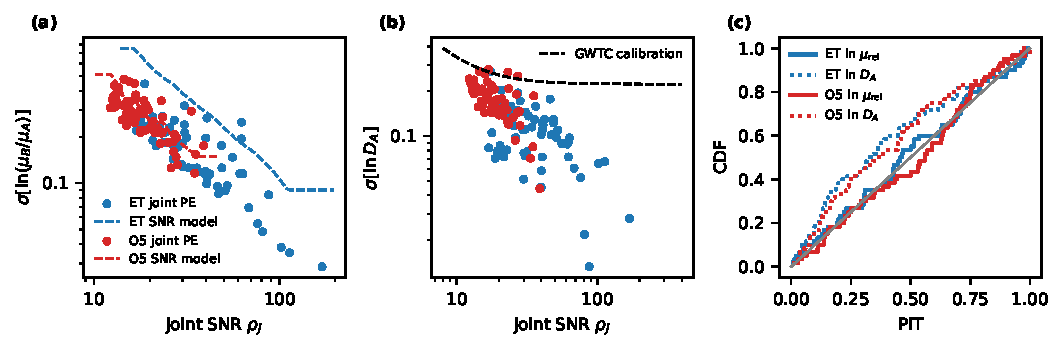
\includegraphics[width=\textwidth]{figures/fig_pe.pdf}
\caption{Joint PE of 120 lensed image pairs from simulated strain. (a) Posterior standard deviation of $\ln(\mu_B/\mu_A)$ versus joint network SNR, with the SNR-based model (dashed). (b) The same for the apparent distance of image $A$, with the GWTC-calibrated error model. (c) Distribution of the probability integral transforms of the truth (diagonal: perfect calibration). ET uses the host sky position, O5 a free sky position.}
\label{fig:pe}
\end{figure*}

\subsection{Bayesian GW+EM lens reconstruction}
\label{sec:gwem}
For the same systems we reconstructed the lens with a conventional likelihood. The lens model is the simulated family (SIS, SIE, SIE+shear or EPL+shear), evaluated with \textsc{lenstronomy}, and its priors are the simulated population distributions: the SLACS-like axis ratio, the log-normal external shear, $\gamma'\sim\mathcal N(2.08,0.15)$ and the $\sigma_v^4$-weighted velocity-dispersion function. The EM likelihood contains the image positions, with the source position integrated out analytically after linearising the lens equation around each observed image, the lens-light axis ratio and orientation, the velocity dispersion through the SIS normalisation, and the lens-light centre. The GW likelihood depends on the lens only through the magnifications, arrival order and Morse indices of the two GW images. We use it in two ways.

\emph{Two-stage analysis.} The joint-PE posterior of Section~\ref{sec:jointpe} is summarised by a Gaussian in $(\ln\mu_B/\mu_A,\ln D_{{\rm app},A})$, after reweighting the samples to remove the distance prior, together with the posterior probabilities of the nine Morse-index combinations. This product is multiplied by the EM likelihood and sampled over the lens parameters only. It is analogous to the effective GW likelihood of \citet{uronen2026silmarel}.

\emph{Full analysis.} The strain likelihood of both images and the EM likelihood are sampled simultaneously, with the source parameters and the lens parameters free. This makes no approximation to the GW likelihood and is the reference for the two-stage analysis. A run takes 20--40 CPU hours; we performed it for 80 of the 120 systems (10 per family and scenario).

Both analyses are run without a cosmology. The GW amplitude then constrains only the relative magnification, and only the arrival order of the delay is used, so they use the information of the scale-free Geometry+GW(ratio)+FU input set, plus the Morse indices, and are directly comparable with the corresponding NPE. As sensitivity tests we also run the two-stage analysis (i) with the EPL+shear model for all families, (ii) with an external convergence $\kappa_{\rm ext}\sim\mathcal N(0,0.025)$, (iii) in a flat $\Lambda$CDM cosmology in which the observed redshifts give $d_L(z_s)$, so that the GW apparent distance measures $|\mu_A|$ and the delay constrains $(1-\kappa_{\rm ext})D_{\Delta t}$, and (iv) with the astrometric error of the GW-source images increased from 0.01 to 0.03 and 0.1\,arcsec, with matching extra scatter in the simulated positions.

Table~\ref{tab:gwem} and Fig.~\ref{fig:gwem} summarise the results. One O5 system is missing from the two-stage analyses because its catalogue entry could not be reproduced exactly from the stored inputs. Coverages of 40--60 systems carry binomial errors of 0.04--0.06.

\emph{Full versus two-stage.} On the 80 systems with both analyses, which see identical noise, the two-stage posterior median of $\ln\mu_A$ differs from the full one by a median $0.15\sigma$ for ET and $0.05\sigma$ for O5, where $\sigma$ is the posterior width, and by more than $1\sigma$ for 10 and 5 per cent of the systems. The 90 per cent intervals have the same width (median ratio 1.02). The largest differences arise when the free-sky ET PE has settled on a wrong sky position (Section~\ref{sec:jointpe}): for one SIE+shear system the free-sky PE places the sky $110\degr$ from the truth and the two-stage $\ln\mu_A$ is off by 3.5, whereas the full analysis, in which the lens model fixes the Morse indices, and the two-stage analysis with the host sky position both recover it. The Gaussian summary of the GW likelihood is therefore adequate, provided the GW posterior itself is converged.

\emph{Bayesian reconstruction versus NPE.} With the host sky position for ET, the two-stage analysis determines $\mu_A$ to a median 8.1 per cent for ET and 13.7 per cent for O5, against 10.5 and 13.8 per cent for the NPE given the same PE relative magnification. Its 90 per cent intervals are 40--45 per cent narrower, but cover the truth less often (0.80 and 0.90 for the two-stage analysis, 0.85 and 0.87 for the NPE, and 0.80 and 0.88 for the full analysis). The NPE, which analyses a new event in seconds once trained, thus reaches the accuracy of a conventional reconstruction within the scatter of these small samples, with calibrated intervals. The Bayesian intervals for ET under-cover by about $2\sigma$, in the full and the two-stage analysis alike (0.75 for the two-stage analysis of free-sky PE, because of the wrong sky solutions). Possible causes are the truncation of the population priors and the linearised image-position likelihood; we have not isolated the cause with these sample sizes.

\emph{Sensitivity tests.} Analysing every system with the EPL+shear model doubles the ET error to 16 per cent (21 per cent for O5), the price of not knowing the lens family, while keeping coverage at 0.80--0.87, in line with the conservative transfer of EPL+shear priors in Section~\ref{sec:transfer}. An external convergence with $\sigma_\kappa=0.025$ hardly changes the scale-free result, because the radial-slope uncertainty dominates. In $\Lambda$CDM, where the observed redshifts turn the GW apparent distance into a magnification measurement and the delay constrains $(1-\kappa_{\rm ext})D_{\Delta t}$, the EPL+shear error falls to 7.3 per cent for ET and 9.8 per cent for O5; this gain is conditional on the assumed cosmology (Section~\ref{sec:discussion}). Increasing the astrometric error of the GW-source images to 0.03\,arcsec leaves the errors within the sample scatter, although the O5 coverage drops to 0.75; at 0.1\,arcsec they roughly double, to 18--19 per cent, and the intervals under-cover (0.66--0.70), which suggests that the linearised image-position likelihood becomes inadequate for larger positional errors. The magnification of a lensed GW image is therefore only as good as the reconstruction of its position in the host.

\begin{table*}
\caption{Bayesian GW+EM reconstruction of $\mu_A$: median relative error and coverage of the 90 per cent interval. Unless noted, the lens model is the true family and no cosmology is assumed. Indented rows modify the known-sky two-stage analysis for ET and the free-sky one for O5. The NPE rows use the scale-free Geometry+GW(ratio)+FU input set.}
\label{tab:gwem}
\begin{tabular*}{\linewidth}{@{\extracolsep{\fill}}lcccccc@{}}
\toprule
 & \multicolumn{3}{c}{ET} & \multicolumn{3}{c}{O5} \\
Analysis & $N$ & err. (\%) & cov. & $N$ & err. (\%) & cov. \\
\midrule
Full (strain + EM), free sky & 40 & 9.6 & 0.80 & 40 & 14.9 & 0.88 \\
Two-stage, free-sky GW PE & 60 & 9.4 & 0.75 & 59 & 13.7 & 0.90 \\
Two-stage, known-sky GW PE & 60 & 8.1 & 0.80 & -- & -- & -- \\
\quad EPL+shear model & 60 & 16.2 & 0.87 & 59 & 20.6 & 0.80 \\
\quad EPL+shear, $\sigma_{\kappa}=0.025$ & 60 & 15.9 & 0.85 & 59 & 21.4 & 0.80 \\
\quad EPL+shear, $\sigma_{\kappa}=0.025$, $\Lambda$CDM & 60 & 7.3 & 0.88 & 59 & 9.8 & 0.93 \\
\quad GW-image astrometry 0.03 arcsec & 60 & 8.9 & 0.85 & 59 & 9.5 & 0.75 \\
\quad GW-image astrometry 0.1 arcsec & 60 & 17.9 & 0.70 & 59 & 18.7 & 0.66 \\
NPE, SNR-model $\mu_B/\mu_A$ & 60 & 10.8 & 0.85 & 60 & 17.8 & 0.87 \\
NPE, joint-PE $\mu_B/\mu_A$ & 60 & 10.5 & 0.85 & 60 & 13.8 & 0.87 \\
\bottomrule
\end{tabular*}
\end{table*}

\begin{figure*}
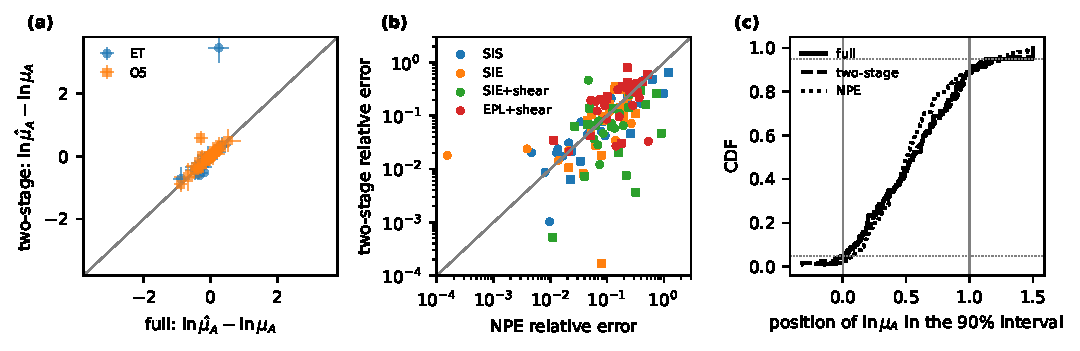
\includegraphics[width=\textwidth]{figures/fig_gwem.pdf}
\caption{Bayesian GW+EM reconstruction. (a) Error of $\ln\mu_A$ from the two-stage versus the full analysis on identical data (free sky). (b) Relative error of the two-stage analysis versus the NPE for the same systems. (c) Distribution of the position of the true $\ln\mu_A$ within the 90 per cent interval (0 and 1 mark its ends) for the full and two-stage analyses and the NPE.}
\label{fig:gwem}
\end{figure*}
